%\documentclass{sig-alternate}
\documentclass[11pt,letterpaper]{article}
\usepackage[margin=1in]{geometry}
\usepackage[doublespacing]{setspace}

\usepackage{amsmath}
\usepackage{amssymb}
\usepackage{framed}
\usepackage{url}
%\usepackage[disable]{todonotes}
\usepackage{todonotes}
\usepackage{graphicx}
\usepackage{float}
\usepackage{tabularx}
\usepackage{fancyvrb}

\newcommand{\acmtitle}[0]{
\title{Nipping Bugs in the Bud\\ Student Mistakes in Introductory Computer Science}
\numberofauthors{3}
\author{
\alignauthor
Nivedita Chopra\\
       \affaddr{Carnegie Mellon University}\\
       \affaddr{Pittsburgh, PA}\\
       \email{niveditc@andrew.cmu.edu}
\additionalauthors{Additional authors: Robert Simmons (Carnegie Mellon University,
email: {\texttt{rjsimmon@cs.cmu.edu}}) and Roy Maxion
(Carnegie Mellon University, email: {\texttt{maxion@cs.cmu.edu}}).}
}
\date{\today}
\maketitle
}

\newcommand{\thesistitle}[0]{
\title{\textbf{\Large{Nipping Bugs in the Bud\\ Student Mistakes in Introductory Computer Science}}}
\author{Nivedita Chopra\\ Advisors : Roy Maxion and Robert Simmons}
\date{}
\maketitle
\thispagestyle{empty}
\clearpage
}

\begin{document}

\thesistitle
%\acmtitle

\presetkeys{todonotes}{color=red!30}{}
\setcounter{page}{1}
\pagenumbering{arabic}

% IEEE bug counts
\def\numlogicIEEE{66 }
\def\numdataIEEE{24 }
\def\numinterfaceIEEE{7 }
\def\numotherIEEE{26 }

% Final bug counts
\def\numlogic{63 }
\def\numdata{21 }
\def\numinterface{7 }
\def\numcomp{32 }
\def\numtotal{123 }
\def\numedge{31 }

\begin{abstract}
\textbf{Background.} Bugs in computer programs may be caused by mistakes in the programmer's thought process. Mitigating the causes of common mistakes in introductory computer science classes can help improve the quality of code that students write in future classes, as well as in industry or academia.\\

\textbf{Aim.} We want to mitigate common mistakes made by students in the Principles of Imperative Computation course (15-122, taught in C0 and C) by analyzing the bugs committed by students in the class, determining the mistakes in thought processes that caused these bugs, and devising ways to correct these mistakes by changing our teaching methods.\\

\textbf{Data.} We collected information about bugs committed by students, including a description of the bug, an optional code snippet, and the student's reasoning behind the bug. This information was collected throughout the Fall 2014 semester (335 students) and during one lab in the Spring 2015 semester (288 students).\\

\textbf{Method.} We classified each bug according to a standard taxonomy (IEEE Standard Classification of Software Anomalies (2010)), determined the mistakes behind common bugs, and proposed ways to mitigate such mistakes.\\

\textbf{Analysis.} We found \numlogic logic bugs, \numdata data bugs, and \numinterface interface bugs per the IEEE standard. An additional category of bugs emerged that we called ``comprehension errors'' (\numcomp instances), which are caused by a misunderstanding of concepts, specifications, or error messages. Among logic bugs, the largest subcategory was due to edge cases (\numedge instances). Edge cases are error conditions occurring at the extremes of operating parameters, perhaps not thoroughly considered by the programmer.\\

\textbf{Pilot Experiment.} With the aim of mitigating mistakes caused by lack of attention to edge cases, we conducted a pilot experiment during one of the weekly labs in the Spring 2015 semester. We split the students in the class into two groups --- a test group and a control group. We encouraged the test group to spend five minutes thinking about edge cases in the assigned problem before beginning to code; the control group received no special instructions.\\

\textbf{Results.} We expected that students who think about edge cases prior to coding would perform better in terms of faster completion times and more incremental progress to solution. When we analyzed the pilot as a full-scale experiment, the analysis yielded a negative result --- the activity did not seem to have any effect on time to completion or on progress toward an error-free solution.\\

\textbf{Conclusion.} The pilot helped us to assess the feasibility of conducting this experiment in a classroom setting and highlighted details in the experimental design that need to be improved upon for a full-scale experiment to be performed in Spring 2016. The negative result is difficult to explain, since we lack evidence as to whether the students actually thought about edge cases. We propose an improved experimental design for Spring 2016 that provides such evidence. Additionally, consistent instructions across lab sessions, and random assignment of students to the two groups, may garner a positive result in the future.
\end{abstract}

\section{Introduction}
\label{sec:intro}

Bugs are a major problem in software development, and bugs in software that is widely used can have far-reaching consequences, as was recently seen in the case of the Heartbleed bug in OpenSSL. While slips in syntax can be detected and fixed easily, oftentimes bugs are caused by mistakes in the programmer's thought process. For example, a student who has misunderstood the workings of pointer arithmetic may add the wrong quantity to a pointer, causing memory errors. Such mistakes ought to be detected and remedied early on, preferably in introductory and intermediate programming classes, to ensure that the programmers of tomorrow are much less likely to commit certain kinds of errors. 

\section{Problem and Approach}
Many mistakes that students make during the course of an introductory computer science course may not be corrected before the end of the semester. Thus students continue to make these mistakes, which may lead to them writing buggy code in higher-level classes and/or industry, where there is no longer a focus on basic computer science concepts.\\

Our approach is to catalog the bugs committed by students in an introductory computer science class. By analyzing these bugs, we hope to gain insight into mistakes in students' thought processes. Based on our analysis, we will devise ways to mitigate these mistakes, such as changing our method of instruction, or changing the way that students think about bugs or about the problems they are solving.

\section{Background and related work}
\label{sec:background}

In the 1980s, much research was aimed at examining bugs committed by students learning to program, and determining flaws in student reasoning from a cognitive standpoint \cite{JoniSolowayGoldmanEhrlich83, PutnamSleemanBaxterKuspa86, SpohrerSoloway86, Pea86}. Much of this work was focused on the student's understanding of specific language constructs such as loops, conditional statements, arrays, etc. \cite{JoniSolowayGoldmanEhrlich83, PutnamSleemanBaxterKuspa86, Pea86}. An example illustrating this is a student misunderstanding of the semantics of a while loop, and making the assumption that the loop condition is being checked at every point within the loop body and not just at the beginning of each iteration of the loop \cite{Pea86}.\\

Most of the work done in the 1980s focused on novice programmers who were learning to program for the first time \cite{SpohrerSoloway86, Pea86}. Our research focuses on students who already know how to program, having taken at least one semester-long programming class. Thus we focus on the students' understanding of algorithms and data structures, and other concepts they are learning for the first time. We also classify the bugs committed by students in the class in a broader sense and avoid focusing on details that are specific to our class and the language in which it is taught (C0 and C).\\

Ko and Myers' work \cite{KoMyers03} classifies and describes errors in programming by linking the errors to their causes. Their model for programming errors is based on Reason's model \cite{Reason90}. Reason's model demonstrates that mistakes in applying knowledge and strategy cause the cognitive problems that lead to errors. Ko and Myers provide a broad taxonomy for errors seen in all types of programming, including both industry and education. Ko and Myers share our goal of connecting errors in programming to mistakes in the programmer's thought process. However, our research focuses on introductory programming classes, and we provide a taxonomy tailored for that purpose.\\

Recently, some research has been done in introductory computer science classes to examine the problems that students face in these classes with an aim of alleviating student frustration and attrition \cite{BryceCooleyHansenHayrapetyan10}. They follow a similar method to ours, of asking students to fill in a form reporting their bugs, yet they differ from our research in two important aspects. Firstly, their classification of bugs is very detailed, with 20 disjoint categories, and focuses heavily on particular concepts and ideas covered in the class, so it is not applicable beyond their class without changes. Additionally, they do not examine student reasoning behind the bug, and classify bugs entirely based on the description and code for the bug.\\

For the purposes of our research, it is important to distinguish between bugs, which are errors based on flawed knowledge, and slips, which are errors based on ``random noise'' \cite{VanLehn90}. While programming, slips are usually manifested as syntax errors and some other errors that may cause a program to fail compilation. On the other hand, bugs are caused by mistakes in the programmer's thought process. In our research, we consider only bugs and we ignore slips entirely. This is because slips in programming are self-correcting, since they almost always cause compile errors which can be easily fixed by the programmer.\\

Our research was performed in an introductory computer science class --- Principles of Imperative Computation (15-122) at Carnegie Mellon University. This class is taught in C0, which is a small safe subset of the C programming language, augmented with contracts \cite{Arnold10, PfenningCortinaLovas11}, and in C. The class introduces computer science students to basic algorithms such as searching and sorting, data structures such as lists, stacks, queues, heaps, trees, etc. and computational ideas such as complexity analysis and proof of correctness of code.


\section{Method}
\label{sec:method}

We recorded bugs committed by the students in Principles of Imperative Computation (15-122) in Fall 2014. Each record of data contained a description of the bug, an optional snippet of the buggy code, and a short explanation by the student of the cause behind the committing of the bug. An example of a record of data is shown in Figure \ref{fig:record}.\\ 

\begin{figure}
\begin{framed}
\emph{What was the bug?}\\
\verb|NULL| pointer dereference\\

\emph{What caused you to write buggy code?}\\
 I did not think of edge cases while writing the code\\

\emph{Include a snippet of the buggy code (optional)}\\
\verb|list = list->next;| //where \verb|list| is \verb|NULL|
\end{framed}
\caption{Example of a record of data}
\label{fig:record}
\end{figure}


Bugs were obtained and recorded in the following ways:
\begin{itemize}
\item{\textbf{Google form.} Students were asked to fill an online form when they found and fixed a bug. In addition to the data points mentioned above, data from this source also contained information on how much time it took the student to find and fix their bug, how they found the bug, and suggestions for how the course staff may have done better in this regard. A screenshot of the form we used is included in Figure \ref{fig:form}}.
\begin{figure*}
\centering
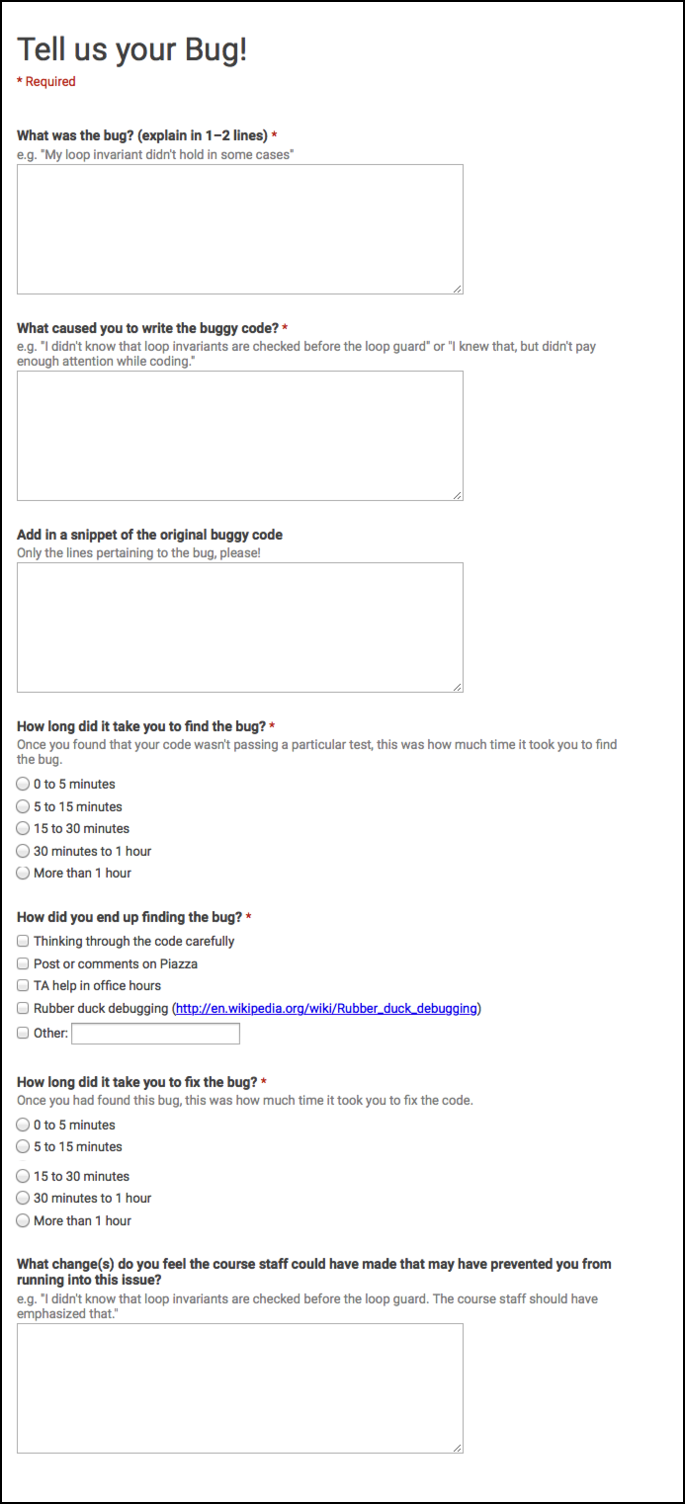
\includegraphics[scale=0.41]{figures/form.png}
\caption{Snapshot of the online Google form that was used to collect data}
\label{fig:form}
\end{figure*}

\item{\textbf{Student observation.} We observed students in labs and office hours and took note of the bugs committed by students in those settings. In this setting, when students fixed their bugs, usually with our help, we asked them to explain their bug and their reasoning behind what caused them to commit the bug.}
\item{\textbf{Piazza.} We analyzed posts made in the online Q\&A forum, Piazza, and recorded the bugs seen there. These posts included a description and/or code pertaining to the bug, and a discussion that led to the bug being solved. We only recorded bugs in which the discussion included student comments that illustrated their reasoning behind the bug.}
\end{itemize}

\begin{table*}
\def\arraystretch{1.75}
\centering
\caption{Error classification by type as per the IEEE Standard Classification for Software Anomalies \cite{IEEE10}}
\label{table:IEEE}
\begin{tabular}{|p{1in}|p{3in}|p{2.4in}|} \hline
\textbf{Type} & \textbf{Description} & \textbf{Example}\\ \hline
Data Error&
Defect in data definition, initialization, mapping, access or use as found in a model, specification or implementation.&
Failure to initialize a variable, modifying data structures during non-destructive operations, dereferencing null, etc.\\ \hline

Logic Error&
Defect in decision logic, branching, sequencing, or computational algorithm, as found in natural language specifications or in
implementation language.&
Incorrect sequencing of code statements, missing cases, performing the wrong operation, etc.\\ \hline

Interface Error&
Defect in specification or implementation of an interface (e.g., between user and machine, between two internal software modules, between software module and database, between internal and external software components, between software and hardware, etc.)&
Use of implementation functions in client code, writing an implementation that does not conform to the interface, etc.\\ \hline

Syntax Error&
Nonconformity with the defined rules of a language.&
Missing semicolon, mismatched parentheses, etc.\\ \hline

Description Error&
Defect in description of software or its use, installation, or operation.&
\\ \hline

Standards Error&
Nonconformity with a defined standard.&
\\ \hline

Other Error&
Defect with no defined type.
&
\\ \hline
\end{tabular}
\end{table*}


With a view towards further examining these bugs, we classified them according to the IEEE Standard Classification for Software Anomalies \cite{IEEE10}. This document provides a standard for classifying anomalies seen during software development. It enables organizations to get insight into the bugs seen during their software development process \cite{IEEE10}.\\

The IEEE standard classifies software anomalies seen in production code on the basis of attributes such as status, priority, severity, probability, effect, type, mode, and insertion activity \cite{IEEE10}. For the purposes of our research, we only care about the classification based on type, as outlined in Table \ref{table:IEEE}.\\


When we classified the collected bugs according to the IEEE standard, we noticed that bugs fell into the logic error (\numlogicIEEE instances), data error (\numdataIEEE instances) and interface error (\numinterfaceIEEE instances) categories. \numotherIEEE instances were categorized as other errors, with no defined type. Three logic errors and three data errors were later reclassified as comprehension bugs (Section \ref{sec:comprehension}).\\

None of our bugs fell into the other three categories of the IEEE standard --- syntax error, description error and standards error. As explained in Section \ref{sec:background}, syntax errors are slips by the programmer, and not bugs, hence they do not appear in our taxonomy of bugs. We do not encounter description errors as we operate under the assumption that the specification provided to students does not contain errors, since it has been thoroughly playtested by the course staff. Additionally, we do not deal with standards, hence standard error is irrelevant.\\

By examining the reasoning provided by students, we realized that we could classify all the bugs that fell into the ``other'' error category of the IEEE standard as ``comprehension errors,'' which are described in the next section.

\section{Comprehension Errors}
\label{sec:comprehension}

While classifying bugs seen in our research, we developed a new category of bugs that is not described by the IEEE classification. We call this new category ``comprehension errors,'' and we feel that it may be unique to introductory computer science classes. A comprehension error occurs when the bug seen is caused due to a misunderstanding on the student's part. Comprehension errors can be roughly divided into four types.
\vspace{0.06in}

\subsection{Using the wrong algorithm or paradigm}
\label{sec:comp1}
Often when a task is described to students, they are unsure about which paradigm or algorithm to use to accomplish it. They may misunderstand the use cases of certain algorithms and paradigms and attempt to solve the problem using an inappropriate algorithm. Figure \ref{fig:comp1} illustrates a comprehension error that involves the use of the wrong algorithm.

\begin{figure}
\begin{framed}
\setlength{\parindent}{0cm}
\textbf{Problem} \\
Find the index of the number \texttt{x} in a given array \texttt{A} containing unique numbers, and return -1 if \texttt{x} is not in \texttt{A}.\\

\textbf{Buggy solution} \\
Use binary search to find \texttt{x} in \texttt{A}.\\

\textbf{Correct solution}\\
Use linear search to find \texttt{x} in \texttt{A}.\\

\textbf{Comprehension error}\\
Binary search cannot be used here since the array is not necessarily sorted. This indicates a lack of understanding of the use case for binary search. We assume that the student correctly understood the specifications.
\end{framed}
\caption{Comprehension error due to using the wrong algorithm or paradigm}
\label{fig:comp1}
\end{figure}

\subsection{Misunderstanding specifications}
\label{sec:comp2}
Students are often unfamiliar with reading specifications, and are hence likely to misunderstand them and to make incorrect assumptions while programming. They may also not understand how to use functions that are provided to help them with generating test cases for their code. Figure \ref{fig:comp2} illustrates a comprehension error that is caused by a misunderstanding of the specifications.\\

The bug illustrated in Figure \ref{fig:comp1} could have been caused by a student's incorrect assumption that the input array is always sorted. If this were the case, the bug in Figure \ref{fig:comp1} would be a comprehension error due to misunderstanding specifications rather than due to using the wrong algorithm or paradigm, as explained in Section \ref{sec:comp1}. In situations like this, we must examine student reasoning behind the bug to determine the correct cause of the bug.

\begin{figure}
\begin{framed}
\setlength{\parindent}{0cm}
\textbf{Problem}
Create the list containing 1, 2, and 4, in order, using the \texttt{cons} and \texttt{nil} functions.\\
\texttt{list cons(int, list); /* Adds the integer to the beginning of the list */\\ list nil(); /* Creates a new empty list */}\\

\textbf{Buggy solution}\\
\texttt{list L = cons(1, cons(2, cons(4)));}\\

\textbf{Correct solution}\\
\texttt{list L = cons(1, cons(2, cons(4, nil())));}\\

\textbf{Comprehension error}\\
Misunderstanding the specification of \texttt{cons} and \texttt{nil}.
\end{framed}
\caption{Comprehension error due to misunderstanding specifications}
\label{fig:comp2}
\end{figure}

\subsection{Misunderstanding error messages}
Due to having limited prior programming experience and possibly because they are using new tools, students are often stumped by error messages and warnings, both from the compiler and from Autolab which autogrades submitted code. Figure \ref{fig:comp3} illustrates a comprehension error that is caused by the misunderstanding of an error message.

\begin{figure}
\begin{framed}
\setlength{\parindent}{0cm}
\textbf{Problem} \\
Perform the bitwise AND operation on two integers \texttt{x} and \texttt{y}.\\

\textbf{Buggy solution} \\
\verb|int z  = x && y|\\

\textbf{Error message}\\
\texttt{:error: type mismatch expected bool found int}\\

\textbf{Correct solution}\\
\verb|int z = x & y|\\

\textbf{Comprehension error}\\
Upon reading the error message, the student thinks that \texttt{x} and \texttt{y} should be booleans rather than integers, because they fail to realize that this error message can also indicate problem with the operator rather than the operands.
\end{framed}
\caption{Comprehension error due to misunderstanding error messages}
\label{fig:comp3}
\end{figure}

\subsection{Lacking clarity on a concept}
When learning a computer science concept, such as integer casting or pointer arithmetic, students may not fully understand the concept, leading them to use these ideas incorrectly while attempting to solve a problem. Figure \ref{fig:comp4} illustrates a comprehension error caused by lack of clarity on a concept.

\begin{figure}
\begin{framed}
\setlength{\parindent}{0cm}

\textbf{Problem}\\
Compute the offset as a signed 16 bit integer that is given as a two-byte operand	to the instruction. Instructions are stored in an array of (unsigned) bytes (\verb|ubyte *P|) \\
 
\textbf{Buggy solution}
\begin{verbatim}
 int16_t o1 = (int16_t)(int8_t)P[pc+1];
 int16_t o2 = (int16_t)(int8_t)P[pc+2];
 int16_t offset = ((o1 << 8) | o2);
\end{verbatim}

\textbf{Correct solution}
\begin{verbatim}
 int16_t o1 = (int16_t)(int8_t)P[pc+1];
 int16_t o2 = (int16_t)(uint16_t)P[pc+2];
 int16_t offset = ((o1 << 8) | o2);
\end{verbatim}

\textbf{Comprehension error}\\ 
Casts both \verb|o1| and \verb|o2| into signed integers to make resultant offset signed. Sign extension on \verb|o2| may alter the final quantity. This shows a misunderstanding of the concept of sign extension.

\end{framed}
\caption{Comprehension error due to lack of clarity on a concept}
\label{fig:comp4}
\end{figure}


\section{Analysis}
\label{sec:analysis}

The bugs observed were logic bugs (\numlogic instances), data bugs (\numdata instances), and interface bugs (\numinterface instances), as per the IEEE Standard Classification for Software Anomalies. An additional category of bugs, with \numcomp observed instances, emerged here that was not specified in the IEEE classification. These are what we have called ``comprehension errors'' (Section \ref{sec:comprehension}).\\

For the bugs that were frequently observed every week, we sought the student misconceptions that may have led to that bug. Since we possessed a timestamp for each bug recorded, we could pinpoint the context in which the bug was made, based on the material covered and assignments due around that time. The reasoning provided by the students, as described in our data collection process in Section \ref{sec:method}, often gave us an insight into the misconception that caused them to write that bug. In other cases, we employed the method of ``just-so stories,'' \cite{JoniSolowayGoldmanEhrlich83} which tries to reconstruct the thought process that may have led to a particular bug, and provides a convincing hypothesis about the student misconception that led to a particular bug. It is worth highlighting the dangers of using the ``just-so'' method to determine student misconceptions from their code. As discussed in Section \ref{sec:comp2}, the comprehension bug illustrated in Figure \ref{fig:comp1} can be categorized as using the wrong algorithm (Section \ref{sec:comp1}) or as misunderstanding the specification (Section \ref{sec:comp2}).\\

\begin{table*}
\def\arraystretch{1.75}
\centering
\caption{Proposed Bug Taxonomy}
\label{table:new-taxonomy}
\begin{tabular}{|p{0.95in}|p{1.6in}|p{2in}|p{2.1in}|} \hline
Type&Example : Instructions&Example : Buggy Code&Example : Correct Code\\ \hline
Logic Bug
& 
Traverse through a linked list performing a certain	operation on each element
& 
\begin{verbatim}
while (li->next != NULL){   
 //do something;
 li = li->next; 
}
\end{verbatim}
& 
\begin{verbatim}
while (li != NULL){   
 //do something;
 li = li->next; 
}
\end{verbatim}\\
\hline
Data Bug
& 
Write a function to check if a given integer is in a linked list
& 
\begin{verbatim}
bool is_in(list L, int n){
 while(L->start != NULL){
  if(L->start->data == n)
   return true;
  L->start = 
           L->start->next;
 }
 return false;
}
\end{verbatim}
& 
\begin{verbatim}
bool is_in(list L, int n){
 list temp = L->start;
 while(temp != NULL){
  if(temp->data == n)
   return true;
  temp = temp->next;
 }
 return false;
}
\end{verbatim}\\
\hline
Interface Bug & 
Write a function that removes the green component of a given pixel
\vspace{0.11in}

\emph{Interface}
\vspace{-0.11in}
\begin{verbatim}
pixel make_pixel(
  int a, int r, 
  int g, int b);
int get_red(pixel p);
\end{verbatim}

\emph{Implementation}
\verb|typedef int pixel;|
& 
\begin{verbatim}
pixel remove_red(pixel p){
   return (p & 0xFF0000);
}
\end{verbatim}
& 
\begin{verbatim}
pixel remove_red(pixel p){
   int a = get_alpha(p);
   int g = get_green(p);
   int b = get_blue(p);
   return 
    make_pixel(a, 0, g, b);
}
\end{verbatim}\\
\hline
Comprehension Bug & 
Create the list containing 1, 2, and 4, in order, using the cons and nil functions

\verb|list cons(int, list);|
\verb|list nil();|
& 
\begin{verbatim}
list L = 
  cons(1, cons(2, 
              cons(4)));
\end{verbatim}
& 
\begin{verbatim}
list L = 
  cons(1, cons(2, cons(4, 
                  nil())));
\end{verbatim}
\\ \hline
\end{tabular}
\end{table*}

Based on our analysis, we propose a new taxonomy of bugs that occur in introductory computer science classes. This taxonomy has four main categories --- logic bugs, data bugs, interface bugs, and comprehension bugs. See Table 2 for examples of bugs classified by this taxonomy.\\

In addition to the observation of comprehension bugs, we also noticed that a large percentage of bugs were logic bugs at the beginning of the semester, and in later weeks, the frequency of comprehension bugs began to increase. The increasing frequency of comprehension bugs as the semester progressed seems to indicate a correlation with the introduction of new and difficult concepts. It should be mentioned that some of the hardest topics, such as type casting and pointer arithmetic were taught near the end of the semester.\\

We also noticed that some bugs can be classified as per the IEEE classification into logic, data, or interface bugs when we look solely at the code. However, when we hear the student's reasoning behind the bug, we realize that they are actually comprehension bugs caused by a misconception harbored by the student. We noticed that six bugs that were initially classified as logic or data bugs (as per the IEEE standard) were later reclassified as comprehension bugs.\\

While traditional bug taxonomies classify the bugs into orthogonal categories based on a description of the bug (in code or as documentation) \cite{Beizer90}, our taxonomy requires additional information about the student's reasoning in order to decide whether a bug is a comprehension bug. Hence the classification of comprehension bugs is dependent  on the availability of additional information, and shows that when classifying bugs in introductory computer science classes, it is not sufficient to record just the bug itself. In such a setting, it is equally, if not more, important to also record the student's understanding of the bug.\\

We were able to record \numtotal bugs throughout the course of the semester. While it would have been ideal to be able to record a larger number of bugs committed by students taking the class \cite{BryceCooleyHansenHayrapetyan10}, we lacked the resources to perform such widespread data collection.

\section{Edge cases}
\label{sec:edge}

Since logic bugs were our largest category (\numlogic of \numtotal bugs), we decided to examine logic bugs more closely. We noticed that \numedge of \numlogic logic bugs (about 50\%) arose due to lack of attention paid to edge cases. Additionally, six out of 31 (about 20\%) of the bugs recorded during one of the weekly labs (discussed in Section \ref{sec:lab}) were related to not checking edge cases.\\

Edge cases are error conditions occurring at the extremes of operating parameters, perhaps not thoroughly considered by the programmer. For example, an empty list serves as an edge case in problems involving lists.\\

We examined various educational strategies with the aim of improving our teaching methods to reduce the number of bugs due to lack of attention to edge cases, and were inspired by the idea of test-driven development (TDD). TDD encourages the writing of tests before beginning to code and leads to better understanding of the task because the programmer has to understand the task fully to write correct test cases \cite{ErdogmusMorisioTorchiano05}. We felt that this strategy could be adapted to deal with edge cases --- getting students to think about edge cases before beginning to code would cause them to pay attention to edge cases while coding.\\

We decided to conduct a pilot experiment where students are split into two groups --- experimental and control. In the experimental group, students consider edge cases in the problem for five minutes before beginning to code. The control group is given no special instructions.\\

Our hypothesis was that students who think about edge cases before coding would perform better than students who immediately begin to code. We expected to see faster completion times to finish the assignment and more incremental progress toward a correct solution from students who thought about edge cases before coding.

\section{Rationale for a Pilot Study}
\label{sec:pilot}

We decided to perform our experiment as a pilot study for various reasons.
\begin{itemize}
\item{\textbf{Feasibility.} In recent years, the size of introductory computer science classes at Carnegie Mellon has increased many-fold, making logistics for a class-wide experiment tricky. Additionally, the only similar research done recently in the computer science department at Carnegie Mellon involved designing a new class from the ground up based on research ideas \cite{Blank14}, something that we did not have the luxury to do. Since this was the first experiment in recent years that was aimed at collecting data while students were coding in a classroom (lab) setting, we felt that it was important to attempt to plan our experiment with all the constraints in mind, and use the pilot to evaluate the feasibility of our design.}

\item{\textbf{Drawbacks in experimental design.} We wanted to use the pilot as an opportunity to find drawbacks in our design, which could be improved upon for the full-scale experiment so that we get cleaner results.}

\item{\textbf{Testing data collection and analysis processes.} We wanted to use the pilot as an opportunity to do a run of our data collection process, and of various metrics that we would use to analyze the results.}
\end{itemize}


\section{Lab : Sorted Linked Lists}
\label{sec:lab}

Among all the weekly labs during which we collected data in Fall 2014, we noticed that the largest number of bugs due to edge cases (six out of 31 total bugs) was seen during the sorted linked lists lab. Thus we performed the pilot during this lab in Spring 2015.\\

The sorted linked lists lab defines a structure called a sorted linked list, which is a linked list of integers with a data structure invariant that the list is sorted in ascending order and contains no duplicates. This means that each node in the linked list is strictly smaller than all the nodes following it in the list.\\

Students were asked to write code for checking that an integer is in the sorted linked list. They were instructed to also complete at least one of insertion into or deletion from a sorted linked list. Insertion and deletion for sorted linked lists involve many edge cases, and this makes these tasks suitable for our experiment.\\

We logged student compilation attempts during the lab. Each log contained:
\begin{itemize}
\item{Timestamp}
\item{Identifier to connect compilation attempts by the same student}
\item{Code that was compiled}
\end{itemize}

\section{Measurement}
\label{sec:measurement}

We decided to analyze the data collected in the pilot as we would for a full-scale experiment. We measured two attributes on our data set --- time to completion and progress to solution.

\subsection{Time to completion}
We measured the time taken for students to arrive at a correct solution, which was characterized by code that passes all our test cases.\\

Our labs started at half past the hour every hour (HH:30). To calculate the time to completion for a student, we looked at the timestamp (T) of the first compilation attempt that passes all the tests. The time to completion was measured in minutes as (T - HH:30) where HH was determined as the half-hour mark closest to the timestamp of the first compilation attempt by that student.\\

We expected that students in the experimental group would on average show faster completion times than students in the control group, which would compensate for the extra five minutes that they spent thinking about edge cases.

\subsection{Progress to solution}

We used the number of test cases passed at each compile to compute the probabilistic distance to solution metric, which is an indicator of how close the student is to the solution \cite{SudolRiversHarris12}.\\

To compute the probabilistic distance to solution, we partition the student code into a finite number of states, where all the code in one state is considered equivalent. We decided our states based on the behavior of student code when compiled and run on an exhaustive test suite. These states are listed in Appendix \ref{sec:appendix-states}.\\

Once we had decided our states, we determined the state of each compilation attempt and noted the transitions between states that corresponded to successive compilation attempts by the same student. Using the states and transitions, we plotted transition state graphs for the experimental and control groups (as depicted in Figures \ref{fig:trans-exp} and \ref{fig:trans-control}). We can perform computations, as described in Sudol, Rivers and Harris' paper \cite{SudolRiversHarris12}, on this transition state graph to determine the probabilistic distance to solution for each of the states. This distance gives us the ability to measure student progress along a path.\\

We expect to see more incremental progress towards the solution from students in the experimental group, who have thought about edge cases. We expect that their initial solution will correctly deal with a larger number of cases than the control group, and that having thought about edge cases will enable them to write better tests and to find the cases for which their code fails.


\subsection{Cyclomatic complexity}

Cyclomatic complexity is a metric for the readability of code \cite{McCabe76}. Lower cyclomatic complexity indicates code that is easier to read and understand.\\

The complexity of a program can be judged by the number of control flow paths through the program. A greater number of loops and conditionals will increase the complexity of a program. Cyclomatic complexity is a graph-theoretic measure of the complexity of the program, and is computed on the control flow graph of the program \cite{McCabe76}. We compute the cyclomatic complexity for the first submission to pass all tests rather than for the final submission because the student may attempt to refactor their code once they have a working solution.\\

We expect to find that the experimental group has written cleaner code with a lower cyclomatic complexity. Since the experimental group kept edge cases in mind from the get-go, they are more likely to have well-structured code that doesn't need a separate case for handling each edge case. On the other hand, the control group would realize that they were missing edge cases only upon failing tests. Thus they were more likely to insert quick fixes in the form of additional cases rather than restructure their code to deal with edge cases in an cleaner manner.

\section{Results}
\label{sec:result}

Our analysis of the pilot as a full-scale experiment yielded a negative result. Performing the activity did not seem to have any effect on the time taken to reach a correct solution or on progress to the solution.\\

\begin{figure}
\centering
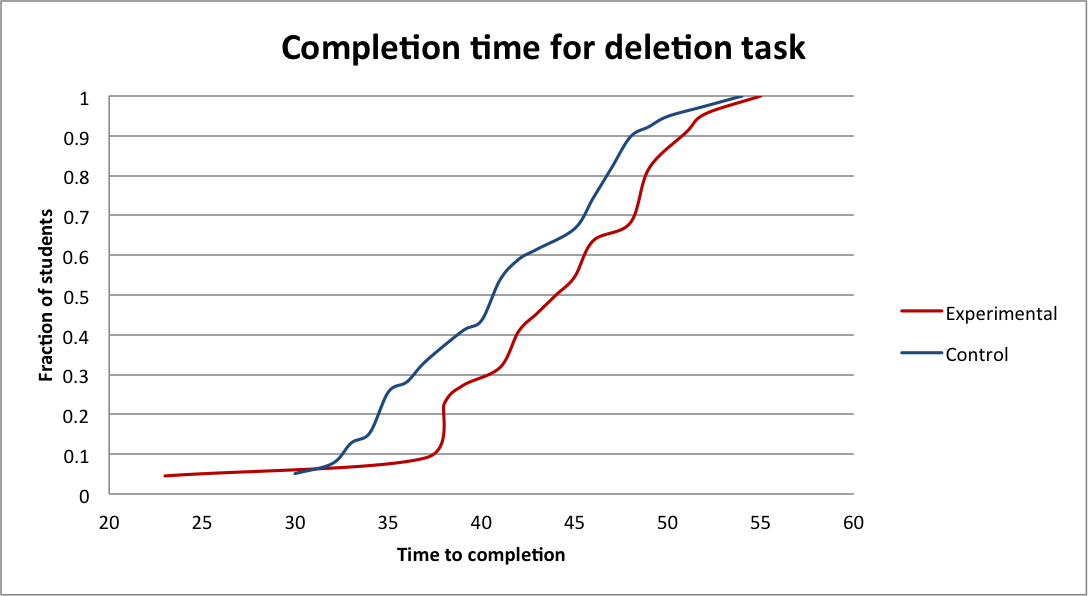
\includegraphics[scale=0.45]{figures/completion-times.png}
\caption{Time to completion for the deletion task between the both groups}
\label{fig:time-result}
\end{figure}

In the experimental group, the five minute activity led to a five minute delay as shown in Figure \ref{fig:time-result}. The median student in the experimental group finished in 44.5 minutes while the median student in the control group finished in 40 minutes, illustrating a 4.5 minute delay. This shows us that students were not able to make up the five minutes that they spent thinking about edge cases before beginning to code.\\

\begin{figure*}
\centering
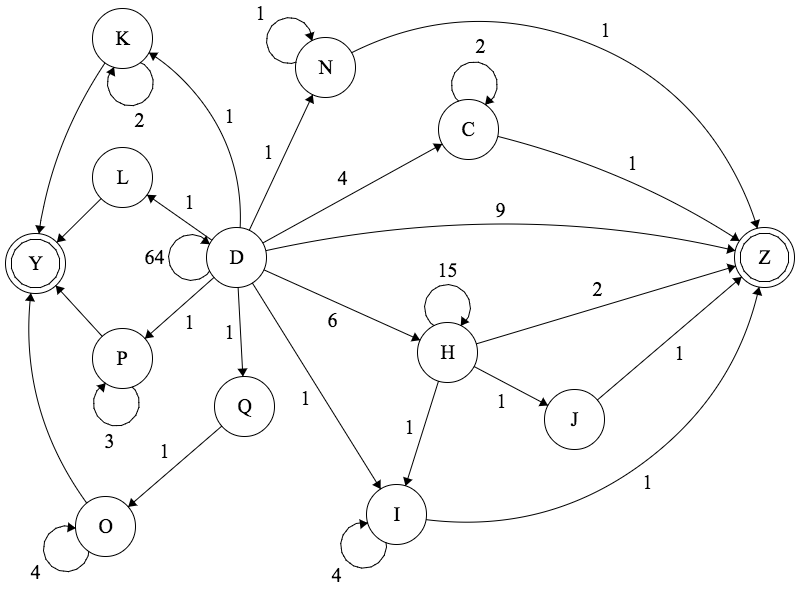
\includegraphics[scale=0.5]{figures/exp-transitions.png}
\caption{Transition state graph for the experimental group for the delete task}
\label{fig:trans-exp}
\end{figure*}

\begin{figure*}
\centering
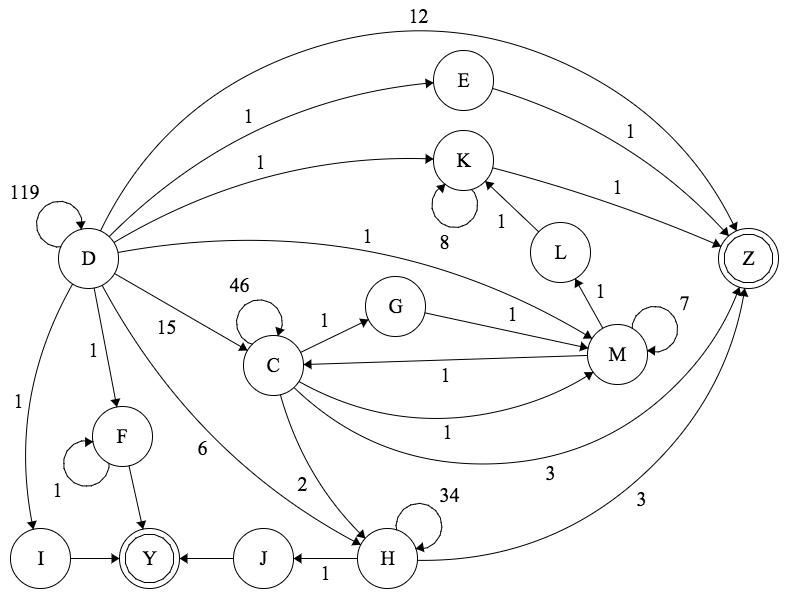
\includegraphics[scale=0.5]{figures/control-transitions.png}
\caption{Transition state graph for the control group for the delete task}
\label{fig:trans-control}
\end{figure*}


We plotted the transition state graph for the two groups, as shown in Figure \ref{fig:trans-exp} (experimental group) and Figure \ref{fig:trans-control} (control group). Each state is characterized by code that passes a certain number and type of tests. In these graphs, D is the start state, and passes only as many tests as the handout code provided to the students. Students leave this state when they pass a different set of tests or their code fails to compile (state B, omitted from the graph) or shows non-termination (state C). Z represents the success state, which is a correct solution that passes all tests, while Y represents a fail state.  States that had no paths to the success state transition to the fail state, thus ensuring that every state has a path to either Y or Z, for the purposes of the probabilitic distance to solution metric computation. A description of all the states can be found in Appendix \ref{sec:appendix-states}.\\

Upon comparing the transitions state graphs for the two groups, we noticed that although some of the paths to the solution differed between the two groups, there were no obvious differences in the length of the path that students followed to the solution. Furthermore, all of the transitions and states that differed among the two groups were followed by only one student, which was not sufficient data to compute a good probabilistic distance to solution metric. We decided to omit all the states that were connected to other states by only one transition. The resulting transition state graph is shown in Figure \ref{fig:exp-filtered} for the experimental group, and Figure \ref{fig:control-filtered} for the control group. The main interesting state is H, which corresponds to missing the edge case of deleting from the beginning of the list. The transition state graph has the same four states for both the control group and the experimental group, and we do not see any obvious differences between the two groups.\\

The cyclomatic complexity metric was not completed in time for the pilot, thus we do not have results for cyclomatic complexity analysis at this time.

\begin{figure}
\centering
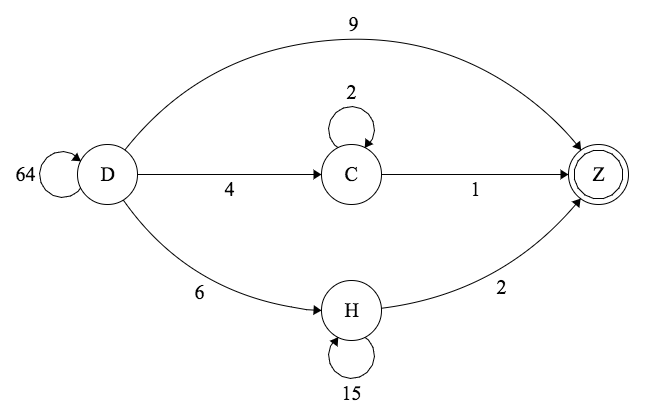
\includegraphics[scale=0.38]{figures/exp-filtered.png}
\caption{Filtered transition state graph for the experimental group for the delete task}
\label{fig:exp-filtered}
\end{figure}

\begin{figure}
\centering
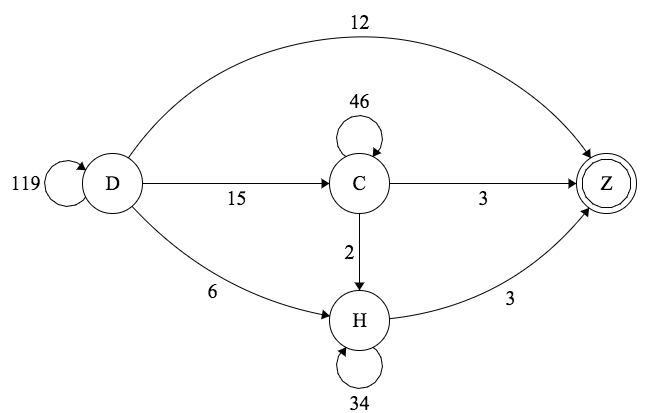
\includegraphics[scale=0.38]{figures/control-filtered.png}
\caption{Filtered transition state graph for the control group for the delete task}
\label{fig:control-filtered}
\end{figure}

\section{What we learned}
\label{sec:learned}

We evaluate our experience in accordance with our rationale for the pilot from Section \ref{sec:pilot}.

\subsection{Feasibility}
We judged that this experiment is feasible in a classroom setting and does not hamper the student's educational experience in any way. Our data collection process involved logging student compilation attempts (as described in Section \ref{sec:lab}) and did not need any additional effort from the students. The control and experimental groups were in separate classrooms, which allowed us to cleanly conduct two separate instances of the same lab. Students were not hampered by the knowledge that some of their classmates were doing the lab with slightly different instructions.


\subsection{Drawbacks in experimental design}

Based on the results of our analysis (as described in Section \ref{sec:result}), we would like to say that thinking about edge cases before coding does not prevent students from commiting bugs due to lack of attention to edge cases. However, we noticed some factors that may have interfered with the experiment which prevent us from making this claim.\\

\textbf{Students may not have grasped the idea of an edge case.}
Instructions to students were based on a previous assignment. Due to restrictions imposed by the Institutional Review Borad (IRB), we were required to keep subjects' identities anonymous, and hence we could not ascertain that all the students had successfully completed that previous assignment. We need some form of feedback on whether students understood the task of thinking about edge cases, which we might get by asking them to list the edge cases for the given problem, either or on paper or in a comment in the file.\\

\textbf{Students may not have thought about edge cases for five minutes.} 
We instructed the students to think about edge cases for five minutes and monitored that they were not coding during that time. However, we also needed some evidence that students actually thought about edge cases. We felt that asking the experimental group to perform an additional task like writing their thoughts on paper might influence their performance and lead to biased results. Thus, constraints on the design of our task prevented us from collecting evidence that the students thought about edge cases for five minutes.\\

\textbf{The instructions may not have been consistent across sessions.}
Another constraint on our experimental design was that an entire classroom was either an experimental group or a control group, and that different groups were led by different TAs, who gave the initial instructions in their own words based off of a general idea. Most TAs led multiple groups throughout the day, and it is likely that the instructions were influenced by the TA's past experience or lack thereof. In the words of one of the TAs, ``By the third time, I knew exactly what to say.'' This can be easily fixed by having pre-tested written instructions for the TAs.\\

\textbf{The participant selection process may not have been random.}
The sections were rigidly predetermined, so there was no opportunity to do random selection of participants for the two groups. Additionally, some sections have a higher concentration of computer science majors than non-majors, and we cannot mix them evenly or select them at will. This is a confounding factor in our experiment and leads to a non-random sample.\\

The fact that these flaws in our experimental design led to our inconclusive results has taught us the importance of good experimental design. We think that it is important for educators to collaborate with people who are familiar with experimental design and methodology to come up with a waterproof design that is free of such issues.

\subsection{Testing Data Collection and Analysis Processes}
Our data collection process was executed without problems. Our metrics for measurement, as described in Section \ref{sec:measurement}, were also tested successfully with the exception of cyclomatic complexity, for which the implementation was not complete at the time of the pilot.

\section{Proposed Next Experiment}
\label{sec:next}

Based on our experiences, as described in Section \ref{sec:learned}, we have designed an improved experiment, that will run as a pilot in Summer 2015 and as a complete run in Spring 2016.\\

We will work towards the same goal of reducing the number of bugs caused by lack of attention to edge cases. We will conduct a similar controlled experiment for which we will split the students into two groups, and we will perform this experiment in the same weekly lab, described in Section \ref{sec:lab}.\\

The control group will spend five minutes writing test cases for the task before beginning to code, in the spirit of test-driven development, as described in Section \ref{sec:edge}. A handout will be provided to students in the control group, which describes a simple problem and exhaustive test cases for that problem. The control group will not be given any special instructions regarding edge cases.\\

The experimental group will also spend five minutes writing test cases before beginning to code. They will be asked to separate their test cases into two groups based on whether or not the test case tests an edge case. The same handout that was provided to the control group will be provided to the experimental group, with one change --- the test cases for the given example will be marked to indicate whether or not they deal with an edge case.\\

Our new design ensures that we get feedback about the edge cases that the student has thought about, in the form of test cases for these edge cases. Additionally, by listing the edge cases for the example in the handout, we ensure that the students are given sufficient explanation of an edge case, and we can also judge their understanding by examining their list of tests for edge cases.\\

We expect to see that students in the experimental group will cover more edge cases in their tests, which may translate to more edge cases covered in their code. We also expect to see faster times to completion and more incremental progress to a correct solution for the experimental group.\\

We can also compare the data we gather from the control group in this experiment to the data collected from the control group in the pilot in Spring 2015 (the experiment that we have described in Section \ref{sec:lab}) to judge the effect of test-driven development. If we see faster completion times and more incremental progress to solution for our new design, we can judge that test-driven development has a positive effect.

\section{Further Work}
It might be useful to get a larger subset of data about bugs seen in the class. One way to do this can be requiring students to complete a form about their problem before and after recieving help at office hours, which is where teaching assistants provide one-on-one help with the programming assignments. Not only will this give us a reliable and larger data source, but it can also help improve the student and TA experience at office hours. Firstly, requiring students to document their problem before recieving help can help discourage many vague questions that TAs often get about the assignment, and force students to think harder about the assignment before asking for help. Secondly, asking students to include their code in the report, can allow the TAs to download the code on their own computer which may help them determine the bug more easily.\\

Since conceptual bugs are more widely seen near the end of the semester, it would be useful to do a more in-depth analysis of these bugs. This could give an insight into concepts that may need to be emphasized in lectures, quizzes, etc.\\

A way to programmatically ascertain whether a given snippet of code contains a logic, data, interface or comprehension error, can help teaching assistants to provide better quality of help to students. This can also be adapted into a system that will provide a student with hints about their error when the student inputs their code and reasoning. Similar tutors have been created for helping novice programmers. They analyze the student code to determine whether the code contains the appropriate algorithms and program components for a given problem, and provides hints based on which components are missing or incorrect \cite{Sudol-DeLyser14}. While this approach works well for analyzing novice code, as we mentioned in Section \ref{sec:analysis}, it's important to also take into account the student's reasoning behind the bug, as the same snippet of buggy code can be written due to different reasons.\\

Another idea would be to correlate student grades and performance with the bugs that the students commit. This might help us predict future performance for students if we know the kind of bugs that they are likely to commit in the future.\\

\section{Conclusion}

In this paper, we aimed to take some first steps towards mitigating mistakes in introductory computer science classes. Our approach was to document the bugs seen in an introductory computer science class throughout the course of a semester. Our categorization and analysis of those bugs showed that a category of bugs called comprehension errors is prevalent in introductory computer science classes. Since comprehension errors highlight a particular concept that was misunderstood by the student, they can provide useful information on concepts that need to be explained better.\\

The observation of a large number of errors due to edge cases encouraged us to conduct a controlled pilot experiment which asked students to think about edge cases for a problem before they begin coding. The pilot helped us to assess the feasibility of conducting this experiment in a classroom setting and highlighted details in the experimental design that need to be improved upon for the full-scale experiment to be performed in Spring 2016. We proposed an improved experimental design that provides such evidence (Section \ref{sec:next}). Additionally, consistent instructions across lab sessions, and random assignment of students to the two groups, may garner a positive result in the future.

\section{Some thoughts}
This senior thesis has been my first venture into research. While helping students as a teaching assistant for 15-122, I noticed that the same types of bugs kept showing up across assignments and semesters. I wondered if there was something we could do better from a teaching perspective to prevent students from running into some of these errors and this led me to pursue this problem as a senior thesis. My main take-away has been that while examining bugs in introductory computer science classes, it is important to also examine the student's reasoning behind the bug.\\

The persistence of comprehension bugs encouraged me to conduct weekly `conceptual office hours' where students could ask questions about any concepts in the class that they felt they had not grasped. Our regular office hours are usually focused on helping students with homework and have long wait times, so these office hours provided a venue for students to improve their understanding of concepts discussed in the class.\\

This research has also influenced the way in which I help students. When helping a student with a problem, I have found that it is best to give them hints by way of asking them smaller questions that point them in the right direction. When a student makes a mistake or answers a question wrong, I resist the urge to say, ``That is not quite right because...'' and instead say, ``Why do you think that is correct?'' This gives me an insight into the student's thought process and helps me mitigate their misconceptions about the concepts being taught in the class.\\

My research has helped me realize that performing educational experiments in established educational settings is very challenging, but also very rewarding. Some challenges arise from the need to perform these experiments within the current framework of the course without hampering the student experience and their learning. Additionally, there is no opportunity to repeat a failed experiment within the same semester because most interventions are coordinated with the teaching of some concepts. Our experiment highlights this because it is reliant on the sorted linked lists lab, which is the only lab that has tasks replete with edge cases. The rewards of doing this kind of research are that it helps us make more educated, data-driven decisions regarding the class curriculum and our teaching practices.

\bibliographystyle{alpha}
%\bibliographystyle{abbrv}
\bibliography{mybib}
%\balancecolumns
\appendix
\section{States in the transition state graph}
\label{sec:appendix-states}
This is an explanation of what each state corresponds to, based on the behavior of the code when compiled and tested against various test cases. The important states are bolded.

\begin{table}
\def\arraystretch{1.75}
\centering
\label{table:trans-states}
\begin{tabular}{|p{0.5in}|p{3in}|} \hline
 \textbf{State} & \textbf{Description}\\ \hline
A & Compile error\\ \hline

B & Runtime error\\ \hline

\textbf{C} & \textbf{Nontermination}\\ \hline

\textbf{D} & \textbf{No effect}\\ \hline

E & Deletion at the beginning and end doesn't work\\ \hline

F & Deletion works on nodes that are neither beginning nor end\\ \hline

G & Only deletion at end works\\ \hline

\textbf{H} & \textbf{Deletion at beginning doesn't work}\\ \hline

I & Deletion at end doesn't work\\ \hline

J & Deletion from beginning of a non-singleton list doesn't work\\ \hline

K & Only deletion at the beginning of non-singleton list works\\ \hline

L & Only deletion at the beginning of non-singleton list and the operation empties the list\\ \hline

M & Deletion works on all lists of length $<= 2$, but cannot delete from middle of list of length $>= 3$\\ \hline

N & Only deletion from the beginning of a non-singleton list works  (all singleton lists work)\\ \hline

O & Deletion of an element from a list of length $>=3$ deletes the entire list after it\\ \hline

P & Fails only the case of deletion of second element of a list of length $>= 3$\\ \hline

Q & Cannot delete from end of a non-singleton list\\ \hline

Y & Failure state (no students reached solution once they entered this state) \\ \hline

\textbf{Z} & \textbf{Success state (this solution passes all tests)}\\ \hline
\end{tabular}
\end{table}

\end{document}

